\newchapter{Introduction}{Introduction}{An Introduction to Self-interacting Dark Matter and Merging Galaxy Clusters}
\label{chapter:1}

Chapter abstract text

%--------------------------------------------------------------------
\section{Composition of the Universe}\label{section:CompositionOfTheUniverse}

Over the past one-hundred years there has been a revolution in our understanding of the universe.
From believing that the Milky Way was the extent of the Universe, the age of Universe was infinite, and that the Universe was composed entirely of atomic matter and photons (cite Hoyle 1950 book).
To now having evidence that the Universe at least extends as far as light can travel in the finite age of the universe ($\sim XXX \pm YYY$), and is dominated by mysterious dark energy and dark matter rather than atomic matter.
Our studies of the universe have improved to such a degree that we are now able to quantify the composition of the universe to percent level accuracy. 
We find that atomic matter (which is dominated by baryonic particles, i.e. particles of the atomic nuclei) only accounts for $\sim$5\% of the universe's total matter-energy budget.
The universe appears to largely be composed of dark matter (DM; $\sim$26\%) and dark energy \citep[$\sim$69\%; see][for more accurate values]{Collaboration:2013uv}.
Very little is known about each of these components.
In very basic terms, dark energy appears to be a particle or field that acts to make the universe expand, while DM appears to be a particle that currently has only been observed to interact via the gravitational force (CDM).
This has come be known as the concordance cosmological model ($\Lambda$CDM).
This dissertation will focus on our efforts to further our understanding of DM, in particular to ascertain whether DM interacts with itself other than through the gravitational force or if it really is just CDM.

%--------------------------------------------------------------------
\section{Dark Matter}

\subsection{Historical Review}

``Dunkle (kalte) Materie'' (or ``Dark (cold) Matter'') was first proposed by Fritz Zwicky in 1933 \citep{Zwicky:1933ub}.
Zwicky had measured the velocities of the galaxies in the Coma galaxy cluster, via their spectroscopic redshifts, and found that given the large velocities the galaxies should not be gravitationally bound if galaxies/stars make up the entirety of the cluster mass.
According to his calculations the total cold dark matter (CDM) mass must be about 400 times that of the mass of the visible galaxies. 
As \citet{vandenBergh:1999jf} notes in his review article, had Zwicky used the correct value for the Hubble constant (rather than H$_0$=558\,km\,s$^{-1}$\,Mpc$^{-1}$) he would have found that the CDM mass must be about 50 times that of the mass of the luminous matter, very close to the actual value of $\sim20$ (disregarding the mass of the X-ray emitting intracluster gas that was unbeknownst to astronomers at the time).
Despite Zwicky's pioneering and shocking findings, the idea of DM did not garner much attention until the work of \citet{Rubin:1970gu} on the rotation velocities of stars and gas in spiral galaxies (e.g. the Andromeda galaxy).
This work was very much in the same vein as Zwicky's work on the Coma galaxy cluster. 
Interestingly, Zwicky also introduced another, completely independent, method of measuring the mass of galaxy clusters and coined the term ``gravitational lens effect'' \citep{Zwicky:1937ec}.
Zwicky argued that if his mass estimates of the Coma cluster were correct, then the cluster should be massive enough to distort space-time to such a degree that as light from distant background galaxies travels through the gravitational potential well of the cluster the light will be deflected and the galaxy images will be distorted in a coherent fashion.
Thus by measuring the distortion of galaxies behind a galaxy cluster one could estimate the mass of the galaxy cluster \citep[see Chapter 2 of][for an introduction to weak gravitational lensing]{Courbin:2002wh}.
\citet{Tyson:1990bc} were the first to successfully measure the gravitational lens effect of a galaxy cluster.
They too found that a mass of the luminous matter alone was insufficient to produce the observed effect.

While the aforementioned work, and subsequent work, found that amount of luminous mass galaxies and clusters was not enough to gravitationally bind the stars and galaxies in those structure, there was still a debate about the solution to this problem. 
Two possible solutions dominated the debate: Zwicky was correct and there existed DM particles, or our understanding of the gravitational force needed to be modified \citep[see][for a review]{Sanders:2002cc}.
This debate remained one of the largest unsettled debates in physics and astronomy until \citet{Clowe:2004eq} published their studies of the Bullet Cluster (1E 0657-558).
The Bullet Cluster was the first discovered \textit{dissociative merger}, see Figure \ref{fig:MergerTimeSeries} for an example of a dissociative merger.
During the merging process the effectively collisionless galaxies  become dissociated from the collisional intracluster gas, which strongly interacts during the merger and becomes pancaked at the point of collision.
In total the cluster gas is about seven times as massive as the gas.
When \citet{Clowe:2004eq} measured where the total cluster mass was with the gravitational lens effect they found that the majority of the mass was located with the galaxies rather than with the gas.
They then inferred that this was only possible if there was a DM particle that was nearly collisionless like the galaxies; modified gravity could not easily explain such an observation.

\subsection{General Properties of Dark Matter}

For a nice review of our current understanding of DM I recommend \citet{Peter:2012tg}, however I will summarize a few relevant points here.
In addition to the abundance of DM (see \S \ref{section:CompositionOfTheUniverse}) there are a few things we know about the properties of DM.
Most notably DM is electromagnetically neutral.
DM does not interact with photons, either through absorption or emission.
Baryons cannot make up a large portion of DM.
This is know from observations of the cosmic microwave background, large-scale structure of the universe, and abundance of light elements created during big-bang nucleosynthesis.
Nor can DM consist solely of light (sub-keV-mass) particles (e.g. neutrinos). 
Light particles move too fast in the early universe to form the initial density concentrations necessary to seed the cosmic structures observed at later times.
DM is completely outside the realm our Standard Model of Particle Physics.
Thus there is no reason to expect that it only interacts via the known forces.
It is entirely possible that DM interacts with itself via some new dark gauge bosons.
Such DM has been termed self-interacting dark matter (SIDM).

%--------------------------------------------------------------------
\section{Motivation for Studying Self-interacting Dark Matter and Existing Constraints}

\subsection{Early Motivation}

The earliest motivation for studying SIMD came from the \textit{missing satellites problem} \citep[see][for a thorough review]{Bullock:2010uv}.
\citet{Moore:1999ja} and \citet{Klypin:1999ej} were the first to note that the number of Milky Way satellites predicted by $\Lambda$CDM simulations significantly exceeded the number of observed satellites.
In an attempt to resolve this problem \citet{Spergel:2000cb} revived a SIDM model with a large scattering cross-section but with negligible annihilation or dissipation\footnote{Such a SIDM model was first proposed by \citet{Carlson:1992cp} and \citet{Machacek:1994kj} to suppress small scale power of CDM dominated cosmologies.  \citet{deLaix:1995ey} found that while SIDM suppressed the small scale power spectrum in a desirable way it resulted in inconsistencies with the observed properties of galaxies.  The \citet{deLaix:1995ey} objects are no longer valid as they only applied to CDM dominated cosmologies, not $\Lambda$CDM cosmologies.}. 
They found that if the SIDM scattering cross-section ($\sigma_{\rm SIDM}/m_{\rm DM}$) is between 0.45--450\,cm$^2$\,g$^{-1}$ then the expected number of Milky Way satellites could be brought inline with the number of observed satellites.
More recently the Sloan Digital Sky Survey (SDSS) and Sloan Extension for Galactic Understanding and Exploration (SEGUE) have enabled the discovery of a number of new dwarf satellites \citep[see][for a review]{Willman:2010fg}, effectively doubling the number of know satellites.
This in combination with simulations that better quantified the selection function of these surveys has helped to reduce the tension between $\Lambda$CDM and the number of observed satellites.
While the missing satellites problem is not resolved it is not nearly as significant as originally believed.
On a final note, recent simulations \citep{Rocha:2012tr} show that for $\sigma_{\rm SIDM}/m_{\rm DM} \sim 1$\,cm$^2$\,g$^{-1}$ the effects of DM halo evaporation are less than originally estimated by \citet{Spergel:2000cb}'s analytic estimates, especially in the outer radii of parent DM halos where the majority of satellites reside.
%This is in stark contrast to the expectations of warm DM (WDM; $\sim$keV-mass), which was also originally considered as a possible solution of the missing satellites problem. 

\subsection{Early SIDM Constraints}\label{section:EarlySIDMconstraints}

Following the revival of SIMD by \citet{Spergel:2000cb} a number of researchers began to constrain $\sigma_{\rm SIDM}m_{\rm DM}^{-1}$ through several independent observations, in what \citet{Peter:2012vi} has termed the ``Y2K-era constraints''.
The Y2K-era constraints fall into five categories:
1) Those that compare the central density of simulated SIDM halos with those observed across a range of halo mass-scales from dwarf spheroids to galaxy clusters \citep{Hogan:2000ih, Kochanek:2000iw, Yoshida:2000bd, Yoshida:2000gn, Dave:2001hh, Dalcanton:2001jj, Meneghetti:2001en, Colin:2002ku}.
Some finding that SIDM created central density cores (i.e. flattened density profile) that were too large and others finding that SIDM with large cross-sections actually exacerbates the formation of cusps (i.e. sharply peaked density profile).
2) Those that compare the shape (i.e. spherical or elliptical) of simulated SIDM halos with the shapes of observed DM halos \citep{Yoshida:2000bd, Dave:2001hh, MiraldaEscude:2002ev}.
They found that as the SIDM cross-section is increase DM halos become more spherically symmetric and at a certain point elliptical halos, such as those observed in some galaxy clusters, can no longer be formed.
3)Those that compared the amount of substructure in simulated SIDM halos with the amount observed in galaxies and galaxy clusters \citep{Hogan:2000ih, Yoshida:2000bd, Gnedin:2001gd, Colin:2002ku}.
As the SIDM cross-section increases subhalos begin to evaporate in their parent DM halo.
4) Those that estimated the formation of super massive black holes (SMBH) as a function of varying SIDM cross-section \citep{Hennawi:2002kv}.
As the SIDM cross-section is increased the initial seeds of SMBH's can form earlier and more efficiently, at some point the expected number and mass of SMBH's exceeds the observed number and mass.
5) Those that compared and contrasted the observed behavior of DM with collisionless galaxies and collisional gas during the merging process of two galaxy clusters \citep{Markevitch:2004dl}.
This method will be the focus of this dissertation and is discussed in great detail in \S\ref{section:DMconstraintWithMergers}.

Of these early works four constrained the velocity independent $\sigma_{\rm SIDM}m_{\rm DM}^{-1}$ to such a degree that it became astrophysically uninteresting.
\citet{Gnedin:2001gd} obtained a constraint of $\sigma_{\rm SIDM}m_{\rm DM}^{-1}\lesssim 0.3$\,cm$^2$\,g$^{-1}$ with their study of subhalo evaporation in galaxy clusters.
\citet{Yoshida:2000gn} and \citet{Meneghetti:2001en} obtained a constraint of $\sigma_{\rm SIDM}m_{\rm DM}^{-1}\lesssim 0.1$\,cm$^2$\,g$^{-1}$ with their study of the central densities of galaxy cluster.
Finally \citet{MiraldaEscude:2002ev} obtained tightest constraint, $\sigma_{\rm SIDM}m_{\rm DM}^{-1}\lesssim 0.02$\,cm$^2$\,g$^{-1}$, with their study of galaxy cluster halo shapes.
However recent SIDM simulations \citep{Peter:2012vi, Rocha:2012tr} have cast serious doubts on each of these previous constraints.
However in recent SIDM simulations\citet{Rocha:2012tr} find that the previous subhalo evaporation and central density constraints are likely overestimated, and \citet{Peter:2012vi} points out several weaknesses of the \citet{MiraldaEscude:2002ev} work as well as presents contradictory results.
In summary \citet{Peter:2012vi} and \citet{Rocha:2012tr} find that the previous constraints need to be loosened to $\sigma_{\rm SIDM}m_{\rm DM}^{-1}\lesssim 1.0$\,cm$^2$\,g$^{-1}$.
As will be discussed in \S\ref{section:RecentMotivation}  $\sigma_{\rm SIDM}m_{\rm DM}^{-1}$ between $\sim$0.3--1.0\,cm$^2$\,g$^{-1}$ has potentially interesting and desirable astrophysical implications.

%Central density profile (i.e. cores in halo):
%
%Dwarfs density cores: Dave et al. 2001 sigma/m=0.1--10
%Hogan \& Dalconton 2000: substructure and central density cusps
%Cluster central density: Meneghetti et al. 2001
%Dalconton \& Hogan 2001: cores in dwarfs to clusters of galaxies
%Kochanek \& White 2000:  claim that SIDM exacerbates the formation of cusps in galaxy halos
%Colin et al. 2002: structure and substructure of Milky Way-sized halos, velocity dependent cross-section, found catastrophic formation of cusps
%Yoshida et al. 2000a {Yoshida:2000bd}
%Yoshida et al. 2000b {Yoshida:2000gn} sigma/m < 0.1
%
%halos shapes (i.e. elliptical halos):
%
%Halo Shapes: Miralda-Escudé 2002 sigma/m < 0.02
%Dwarfs density cores: Dave et al. 2001 sigma/m=0.1--10
%Yoshida et al. 2000a {Yoshida:2000bd}
%
%Substructure in DM halos / halo evaporation:
%
%Subhalo evaporation: Gnedin \& Ostriker 2001 sigma/m < 0.3
%Hogan \& Dalconton 2000: substructure and central density cusps
%Colin et al. 2002: structure and substructure of Milky Way-sized halos, velocity dependent cross-section, found catastrophic formation of cusps
%Yoshida et al 2000a {Yoshida:2000bd}
%
%growth of SMBH:
%
%Hennawi \& Ostriker 2002 sigma/m $\sim$0.02 (need to investigate this further
%
%Merging Galaxy Cluster
%Merging Cluster: Randall et al 2008 sigma/m < 0.7--1.25
%
%By comparing DM halo shapes and the substructure there in \citet{Moore:2000ee} found that simulations with $\sigma_{\rm SIDM}m_{\rm DM}^{-1}\sim 10$\,cm$^2$\,g$^{-1}$ resulted in halos with singular isothermal density profiles which ``is inconsistent with galactic rotation curves''\footnote{\citet{Moore:2000ee} don't actually define the $\sigma_{\rm SIDM}m_{\rm DM}^{-1}$ they use in their model. Since they treat SIDM as a non-radiative gas I have estimated the cross-section by comparing the scattering depth of such a gas with that of SIDM with a given cross-section \citep[see for example][]{Markevitch:2004dl}}.
%Thus \citet{Moore:2000ee} effectively placed a constraint of $\sigma_{\rm SIDM}m_{\rm DM}^{-1}\lesssim 10$\,cm$^2$\,g$^{-1}$.
%
%Repeat similarly for other constraints... (perhaps too much detail though) and I could just summarize the methods that provide the tightest constraints.
%
%See the summary by \citet{Peter:2012vi} on page 106.

\subsection{Recent Motivation}\label{section:RecentMotivation}

After the burst of Y2K-era work, the field of SIDM essentially died, with only a few new constraints trickling in \citep{Randall:2008hs, Dawson:2012dl, Merten:2011gu}.
However, the field has recently entered a renaissance with extensive theoretical work {ArkaniHamed:2009gk, Feng:2010kh, Tulin:2012jt, Tulin:2013eo, Ackerman:2009ia, Pospelov:2008di} and simulation work \citep{Peter:2012vi, Rocha:2012tr, Vogelsberger:2012dy, Vogelsberger:2013bb, Zavala:2013iq}.
This renaissance can largely be attributed to three apparent conflicts between astrophysical observations and $\Lambda$CDM:

{\it (i)} Studies of the stellar kinematics in low surface brightness (LSBs) and dwarf spheroidal galaxies \citep[dSphs;][]{Simon:2005fu, deNaray:2008iz, Oh:2011jd} have shown that the radial velocity profiles of the stars in many halos are better fit by an isothermal density profile (i.e. cored profile) rather than an Navarro-Frenk-White \citep[NFW;][]{Navarro:1996ce} density profile predicted by $\Lambda$CDM.
In other words $\Lambda$CDM produces DM halos that are too cuspy, while an isothermal density profile suggests that there is energy exchange occurring in the centers of these galaxies.
The simulations \citet{Rocha:2012tr} found that if $\sigma_{\rm SIDM}m_{\rm DM}^{-1} \sim 0.5$\,cm$^2$\,g$^{-1}$ then there is enough thermal exchange between the DM to produce cores of the size observed in the LSBs and dSphs.

{\it (ii)} All observed dSphs of the Milky Way have 12$\leq V_{\rm circ}(r_{1/2} \leq$20\,km\,s$^{-1}$, where $V_{\rm circ}(r_{1/2}$ is the circular velocity of particles at the half-light radius.
The more mass there is within $r_{1/2}$ the larger $V_{\rm circ}(r_{1/2}$.  
Recent $\Lambda$CDM simulations of Milky Way-like halos predict that at least 10 dSphs should have $V_{\rm circ}(r_{1/2} > 20$\,km\,s$^{-1}$ \citep{BoylanKolchin:2012id}.
If the $\Lambda$CDM simulations are correct then this would suggest that Milky Way is missing a significant number of large dSphs, or these large dSphs DM halos are devoid of stars which is entirely implausible.
SIDM of allowable cross-section results in a nearly identical power spectrum at these scales and above \citep{Rocha:2012tr}, thus these large dSphs will still exist in SIDM cosmologies.
While this appears to be an entirely separate problem than the dSphs cusp/core problem previously mentioned, it may just be another perspective of exactly the same problem.
Perhaps it is not that these massive dSphs are missing but rather that their central densities are lower than predicted by $\Lambda$CDM (i.e. they are cored).
If they are cored then some of the halo mass is diffused from the central $r_{1/2}$ outwards.
Thus the halo's mass could remain the same but $V_{\rm circ}(r_{1/2}$ would decrease.
Again the work of \citet{Rocha:2012tr} suggests that if DM self-interacts with $\sigma_{\rm SIDM}m_{\rm DM}^{-1} \sim 0.5$\,cm$^2$\,g$^{-1}$ then the resulting central densities of the dSphs would be cored to such a degree to ameliorate this apparent discrepancy. 

{\it (iii)} Finally on the much larger galaxy cluster scales, recent observations of their density profiles \citep{Newman:2012wt, Newman:2012tk} suggest that the cluster have central cores at odds with $\Lambda$CDM.
Comparison of the observed core size with simulations \citep{Peter:2012vi, Rocha:2012tr} shows that $\sigma_{\rm SIDM}m_{\rm DM}^{-1} = 1.0$\,cm$^2$\,g$^{-1}$ will produce cores larger than what is observed.
However, SIDM with $\sigma_{\rm SIDM}m_{\rm DM}^{-1} \sim$0.1-0.5\,cm$^2$\,g$^{-1}$ is capable of producing the observed cores.

These observations all highlight inconsistencies with $\Lambda$CDM and simultaneously suggest SIDM with $\sigma_{\rm SIDM}m_{\rm DM}^{-1}  \sim$0.1-0.5\,cm$^2$\,g$^{-1}$.
If $\sigma_{\rm SIDM}m_{\rm DM}^{-1}  \lesssim$0.1\,cm$^2$\,g$^{-1}$ then SIDM is not capable of resolving any of these observed inconsistencies.
Given the modified existing constraints of $\sigma_{\rm SIDM}m_{\rm DM}^{-1}\lesssim 1.0$\,cm$^2$\,g$^{-1}$ this leaves a very narrow window of parameter space to explore.

%--------------------------------------------------------------------
\section{Probes of SIDM}

While laboratory experiments have placed tight constraints on the baryon-dark matter interaction cross-section ($~21$ orders of magnitude tighter the the current $\sigma_{\rm SIDM}$ constraints), these experiments are insensitive to dark matter-dark matter interactions.
The only way to investigate whether DM self-interacts is through astrophysical observations (\S\ref{section:EarlySIDMconstraints} summarized the various astrophysical methods for constraining SIDM). 

As discussed in the previous section the greatest tensions with $\Lambda$CDM come from studies of the central densities of DM halos.
This is true over a range of halo scales from LSBs to galaxy clusters.
While such probes suggest that dark matter may self-scatter, each suffers from a \emph{baryonic degeneracy}, where the observations might be explained by various baryonic processes/assumptions (e.g. AGN or supernove feedback, or the assumed initial mass function).
In fact the important scales of these observations often coincide with baryonic scales \citep[e.g. the core size in clusters is approximately the size of the brightest cluster galaxy;][]{Newman:2012wt, Newman:2012tk}.
What is needed is a probe of self-interacting dark matter (SIDM) where the expected effect is independent of these baryonic degeneracies.
Merging galaxy cluster are such a probe. 

%--------------------------------------------------------------------
\section{Merging Galaxy Clusters as Probes of Self-Interacting Dark Matter}

\subsection{Merging Galaxy Clusters}\label{Section:MergingClusters}

According to the generally accepted model of structure formation in the Universe small structures (e.g. galaxies) form first then through gravitational attraction begin to merge and form larger structures (e.g. galaxy clusters).
This process constantly repeats throughout the history of the universe and is known as the hierarchical structure formation model.
When small structures merge with larger structures (e.g. dSphs merging with a galaxy or a galaxies merging with a galaxy cluster) the smaller structures are often dramatically altered (having the stars, gas and DM stripped from them), yet the larger structures remain largely unaffected and there is little net change in the system.
Occasionally structures of nearly the same size (e.g. two galaxies or two galaxy clusters) will merge.
In these cases the system is often dramatically disturbed and will remain in such a disturbed state until dissipative processes (e.g. dynamic friction, and thermal radiation) cause the two structures to combine and the system to enter a relaxed state.
It is the disturbed phase of merging galaxy clusters that provides the best means of testing whether DM self-interacts.

Merging galaxy clusters are the most energetic example of hierarchical structure formation.
Figure \ref{fig:MergerTimeSeries} shows the generic time-series picture of a merging galaxy cluster leading to a \textit{dissociative merger}, a highly disturbed system where the intracluster gas has become dissociated from the galaxies and DM.
In the case of a dissociative merger two subclusters\footnote{While they are both technically galaxy clusters they are termed subclusters to distinguish them from the galaxy cluster system they will eventually form when the merger is complete.} begin with some physical separation, often significantly larger than the size of the individual subclusters.
The mass of each subcluster is composed of $\sim$2\% galaxies, $\sim$15\% intracluster gas, and $\sim$85\% DM.
Through gravitational attraction the two subcluster accelerate towards one another with the relative velocity of each approaching free-fall velocity.
Eventually the two subclusters collide\footnote{The time of collision is defined to be the time of the first pericentric passage ($t_{\rm 4}$ of Figure \ref{fig:MergerTimeSeries}).}
Because there is so much space between the galaxies, a strong interaction between any two galaxies is extremely unlikely and they can be treated as effectively collisionless particles.
And since the galaxies of each subcluster have built up momentum they will pass through and begin to separate (this time on the opposite side; see $t_{\rm 5}$ of Figure \ref{fig:MergerTimeSeries}).
The gas however is more evenly distributed, thus an interaction between the gas particles of each subcluster is more likely.
These interactions will convert some of the infall kinetic energy into thermal energy (i.e. the gas of each subcluster will experience ram pressure), the net effect being that the gas halo of each subcluster is slowed with respect to the galaxies and much of it becomes dissociated remains centered between the galaxies of the two subclusters (`C' in $t_{\rm 6}$ of Figure \ref{fig:MergerTimeSeries}).
Given that $\sigma_{\rm SIDM}m_{\rm DM}^{-1} \lesssim 1.0$\,cm$^2$\,g$^{-1}$, if the DM interacts it will be significantly less than the gas and behave more like the effectively collisionless galaxies.
Thus the DM will predominately be located with the galaxies. 
It is during this disturbed phase of the merger ($t_{\rm 6}$ of Figure \ref{fig:MergerTimeSeries}) that it is termed dissociative and can provide the best constraints on  $\sigma_{\rm SIDM}m_{\rm DM}^{-1}$.  

\begin{figure}
\centering
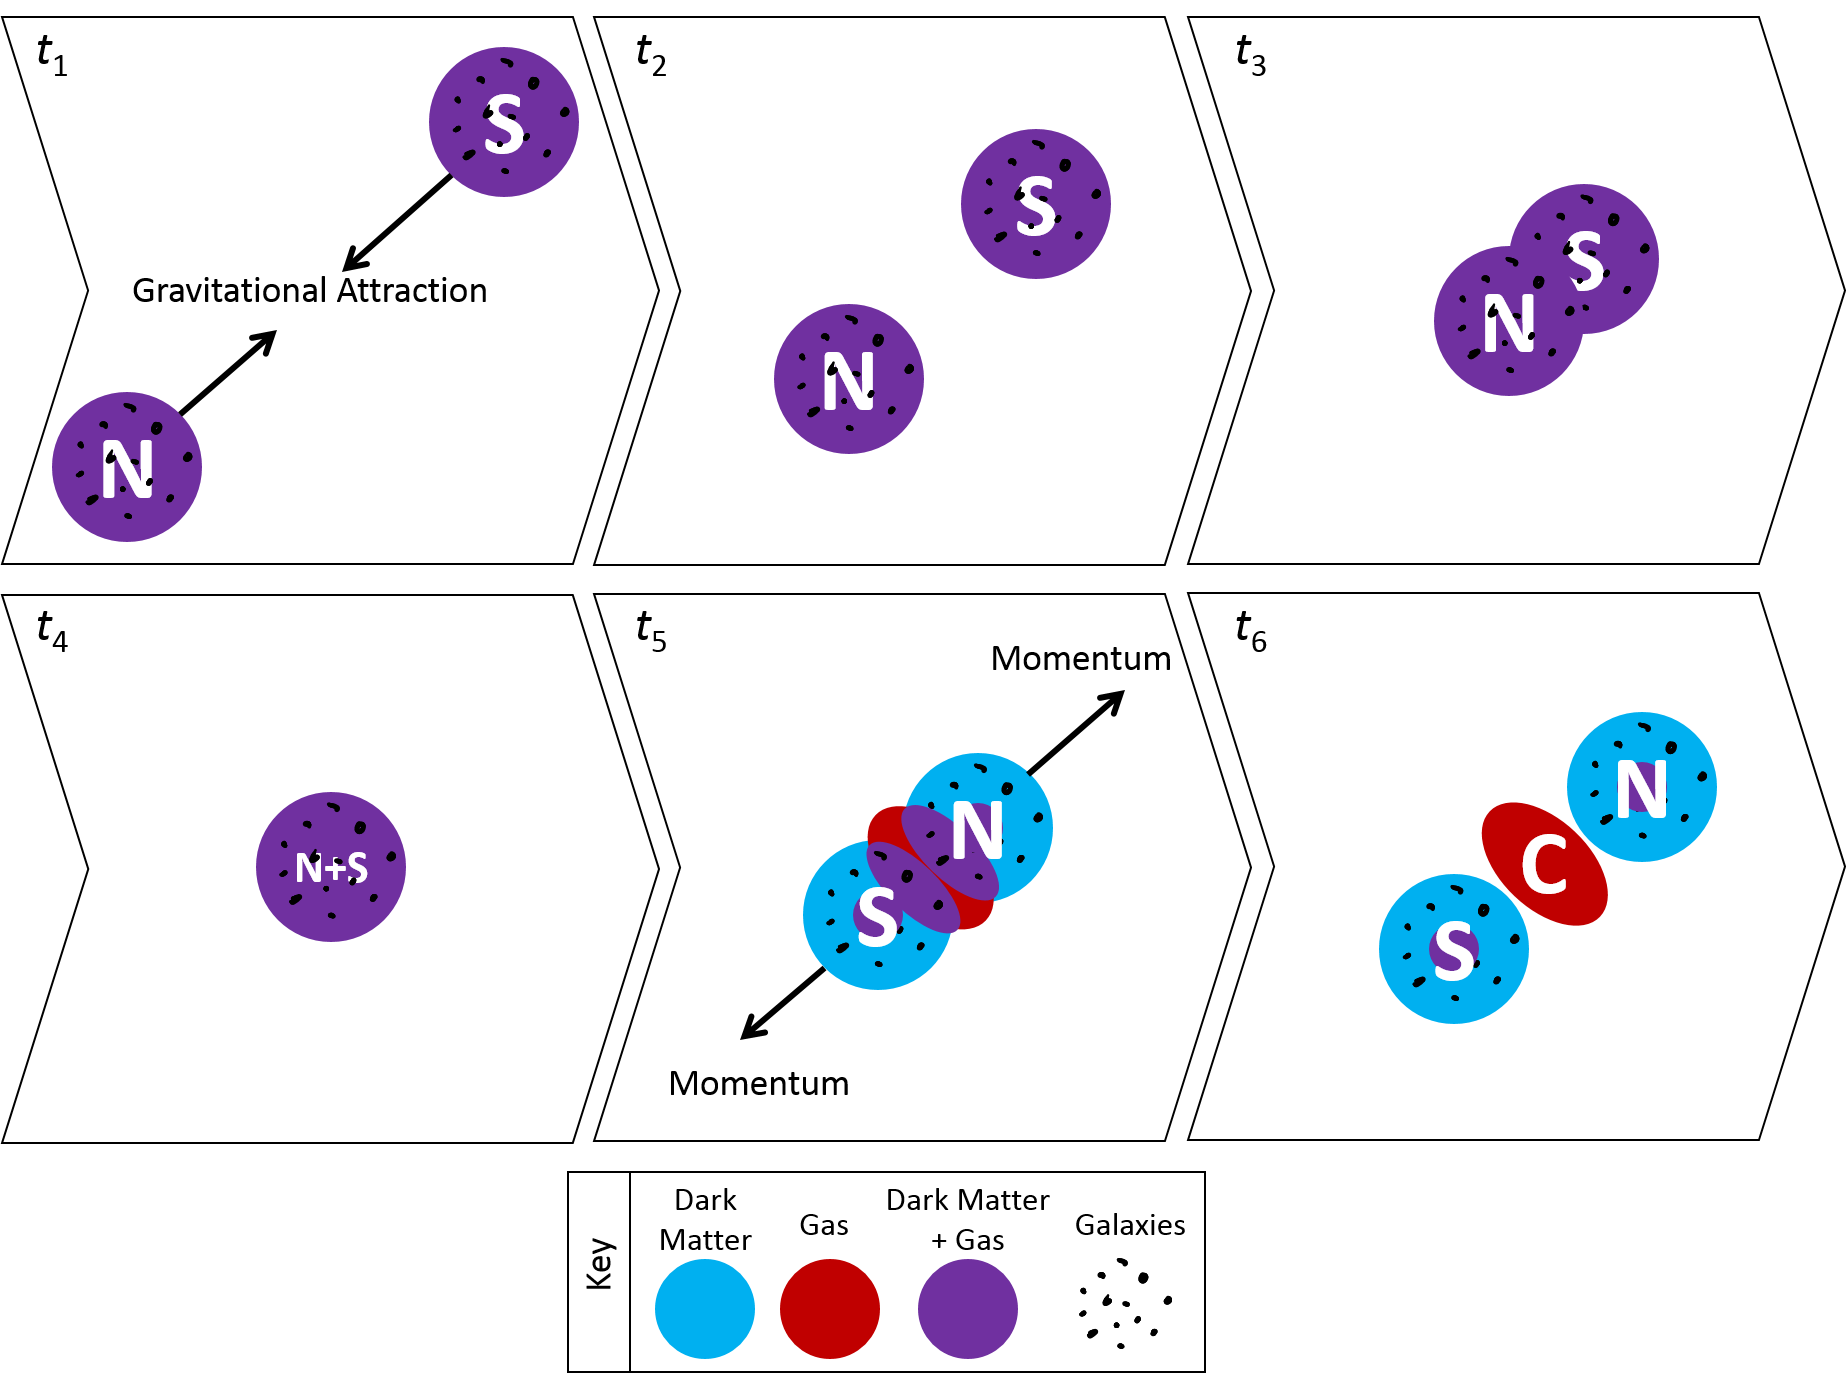
\includegraphics[width=6in]{Chapter1/MergerTimeSeries.png}
\caption[A basic time series leading to a dissociative galaxy cluster merger.]{A basic time series leading to a dissociative galaxy cluster merger (assuming the Standard Model of Cosmology).
Two galaxy clusters (N \& S), each consisting of overlapping halos of DM and gas as well as sparsely populated galaxies, begin with an initial physical separation ($t_{\rm 1}$).
Due to the mass of each galaxy cluster they experience a gravitational attraction and accelerate towards one another until eventually they collide ($t_{\rm 1}$--$t_{\rm 4}$).
By convention time $t_{\rm 4}$ is defined as the ``collision''.
The momentum of the effectively collisionless galaxies will cause them to pass through the impact, $t_{\rm 5}$, only slowed slightly by dynamic friction. 
The collisional gas will strongly self-interact, slowing significantly, and remain in the center ($t_{\rm 6}$ C).
Much like the galaxies the DM behaves in a nearly collisionless manner and appears largely coincident with the galaxies.
Much like the galaxies the DM behaves in a nearly collisionless manner and appears largely coincident with the galaxies.
At $t_{\rm 6}$ the galaxy cluster merger is classed as \emph{dissociative merger}.
At later times dissipative processes (e.g. dynamic friction, and thermal radiation) will have caused the two structures to combine into a single relaxed galaxy cluster.
\label{fig:MergerTimeSeries}}
\end{figure}  

\subsection{Constraining Self-Interacting Dark Matter with Merging Galaxy Clusters}\label{section:DMconstraintWithMergers}

\citet{Markevitch:2004dl} originally introduced (and applied to the Bullet Cluster) three methods for constraining $\sigma_{\rm SIDM}$ with observations of dissociative mergers.
This was followed by \citet{Randall:2008hs} who introduced (and also applied to the Bullet Cluster) an additional method of constraint by combining observations and simulations of dissociative mergers.
These four methods are shown in Figure \ref{fig:4ConstraintMethods} and are discussed below.

\begin{figure}
\centering
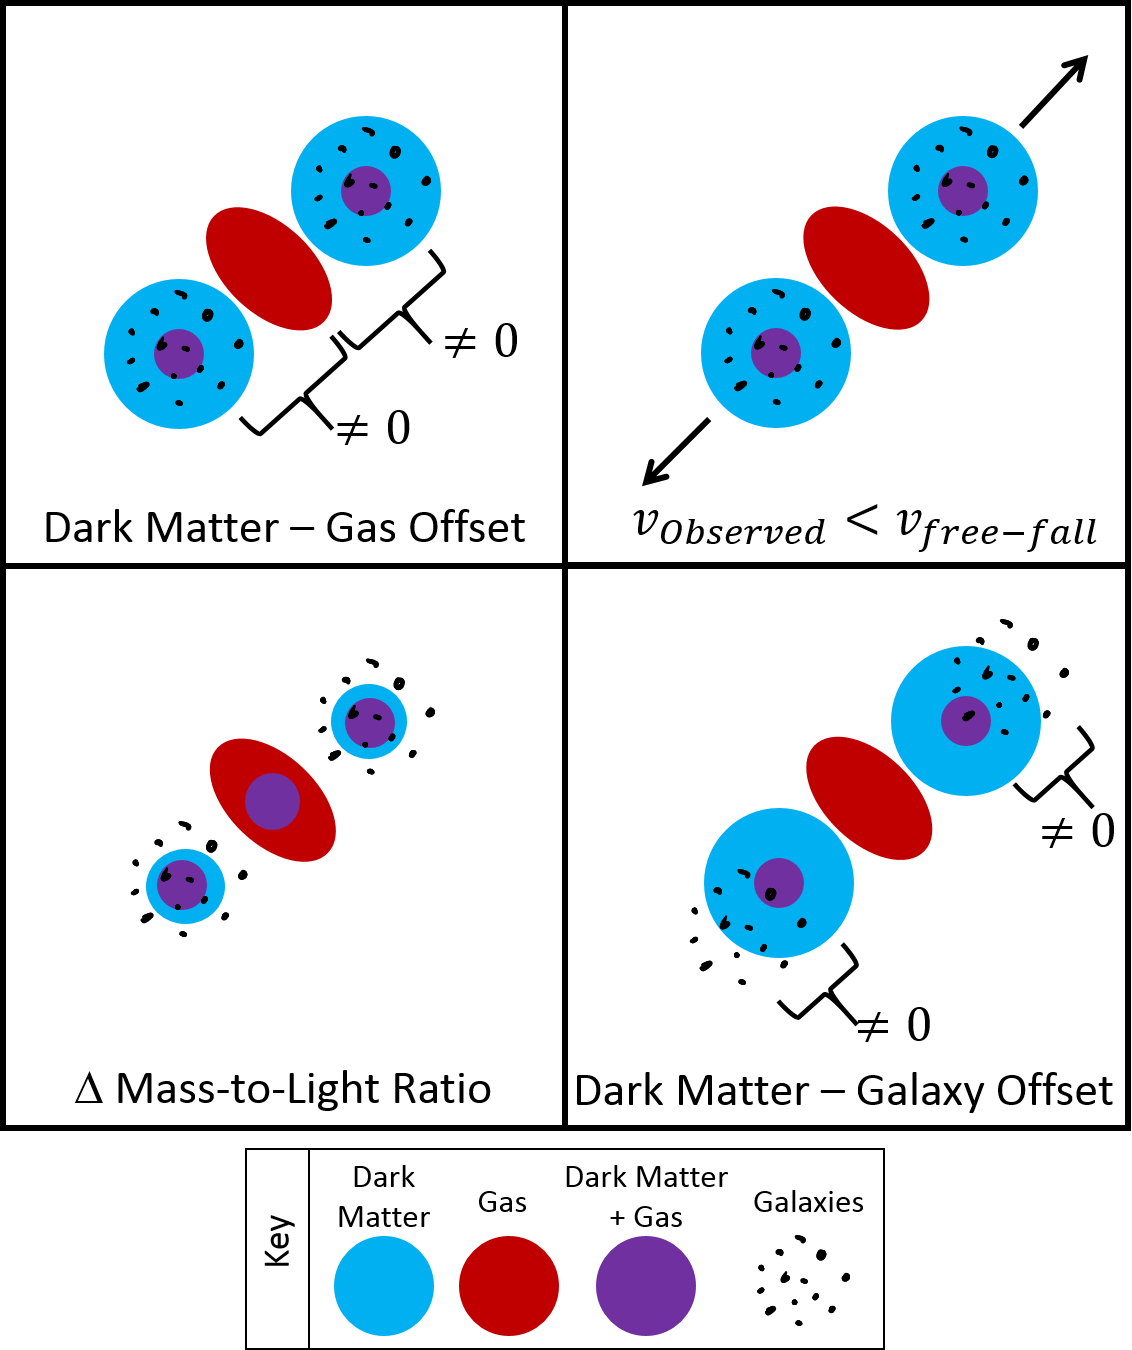
\includegraphics[width=4in]{Chapter1/4ConstraintMethods.png}
\caption[The four means of constraining $\sigma_{\rm SIDM}$ with merging clusters.]{The four means of constraining $\sigma_{\rm SIDM}$ with merging clusters, originally outlined by \citet{Markevitch:2004dl} and \citet{Randall:2008hs}. 
\emph{Upper Left:} If the DM is significantly offset from the gas then the scattering depth of the dark matter ($\tau_{\rm DM}$) must be less than the scattering depth of the gas ($\tau_{\rm gas}$) and an upper limit can be placed on $\sigma_{\rm SIDM}$.
\emph{Upper Right:} If DM self-interacts during the merger, then the velocity of each subcluster will be slowed to some degree.
Thus if the observed velocity ($v_{\rm obs}$) is found to be consistent with the free-fall velocity ($v_{\rm free-fall}$) an upper limit can be placed on $\sigma_{\rm SIDM}$.
If however $v_{\rm obs}$ is significantly less than $v_{\rm free-fall}$, an upper limit could be potentially placed on $\sigma_{\rm SIDM}$.
\emph{Lower Left:} If DM self-interacts during the merger, then some fraction of the DM particles will scatter and become unbound from each subcluster.
Thus the mass-to-light ratio of each subcluster can be compared with the mass-to-light ratio of similar non-merging clusters, and depending on whether the mass-to-light ratio of the merger is the same or less than the non-merging clusters' mass-to-light ratio, then respectively an upper limit or lower limit can be placed on $\sigma_{\rm SIDM}$.
\emph{Lower Right:} If the DM self-interacts during the merger, then the DM component of each subcluster will experience an additional drag force and will travel at a slower velocity than the respective subcluster galaxies.
Thus depending on whether a significant offset between the galaxies and DM is or is not observed, then respectively a lower limit or upper limit can be placed on $\sigma_{\rm SIDM}$.
\label{fig:4ConstraintMethods}}
\end{figure}

\subsubsection{Dark Matter - Gas Offset}
The first method that \citet{Markevitch:2004dl} introduced used the fact that in the case of the Bullet Cluster the DM was observed to be significantly offset from the gas.
According the the generic merger picture discussed in \S \ref{Section:MergingClusters} this is because the collisional gas has a significantly larger scattering depth than the DM and thus is likely to self-interact and become dissociated from the DM.
Thus \citet{Markevitch:2004dl} setup the following inequality relating the scattering depth of the gas, $\tau_{\rm gas}\approx 1$, to the scattering depth of SIDM, $\tau_{\rm SIDM}=\sigma_{\rm SIDM}m^{-1}_{\rm DM} \Sigma_{\rm DM}$.
$\Sigma_{\rm DM}$ is the surface mass density of the DM particles.
\citet{Markevitch:2004dl} assumed that $\Sigma_{\rm DM}$ is approximately the WL measured surface mass density, $\Sigma$, since the majority of a typical cluster's mass is DM.

\begin{displaymath}
\tau_{\rm gas} \gtrsim \tau_{\rm SIDM}
\end{displaymath}

\begin{displaymath}
1 \gtrsim \frac{\sigma_{\rm SIDM}}{m_{\rm DM}} \Sigma_{\rm DM}
\end{displaymath}

\begin{equation}\label{equation:scatterdepth}
\frac{\sigma_{\rm SIDM}}{m_{\rm DM}} \lesssim \Sigma_{\rm DM}^{-1}
\end{equation}

This method has been applied to a number of dissociative mergers \citep{Markevitch:2004dl, Dawson:2012dl, Merten:2011gu}, with constraints ranging from $\sigma_{\rm SIDM}m^{-1}_{\rm DM} <$3-8\,cm$^2$\,g$^{-1}$.
This method has two notable disadvantages that are apparent from Equation \ref{equation:scatterdepth}: the constraint can only be improved by finding clusters with larger $\Sigma_{\rm DM}$ and that the constraint is directly proportional to the inverse surface mass density.
Two of the existing constraints \citep{Markevitch:2004dl, Merten:2011gu} come from extremely dense clusters.
To better the existing $\sigma_{\rm SIDM}m^{-1}_{\rm DM}$ by the necessary order of magnitude would require clusters with surface mass densities an order of magnitude higher than both the Bullet Cluster and Abell 2744.
Such clusters are highly unlikely to exist, thus this method has little value for future constraints of SIDM.
 
\subsubsection{Velocities of the Subclusters} 
 
\citet{Markevitch:2004dl} noted that the Bullet Cluster merger velocity inferred from the X-ray gas shock feature ``is in good agreement with the expected free-fall velocity''.
They then argued that if DM self-interacts then each subcluster will decelerate, resulting in a velocity difference between the observed velocity, $v_{\rm obs}$, and the free-fall velocity, $v_{\rm free-fall}$:

\begin{displaymath}
v_{\rm obs} - v_{\rm free-fall} = \frac{\bar{p}}{m_{\rm DM}}\frac{\sigma_{\rm SIDM}}{m_{\rm DM}} \Sigma_{\rm DM},
\end{displaymath}
where $\bar{p}$ is the average momentum lost by the subcluster in each particle collision.

This method has only been applied to the Bullet Cluster \citep{Markevitch:2004dl}, and resulted in a constraint of $\sigma_{\rm SIDM}m^{-1}_{\rm DM} \lesssim$7\,cm$^2$\,g$^{-1}$.
The predominant reason this method has not been applied to more mergers is that it is very difficult to constrain the three-dimensional velocity of the merger \citep{Dawson:2012ub}, which is necessary to estimate $\bar{p}$.
Often times the only direct observation of the merger velocity comes from spectroscopic redshifts of the subcluster galaxies, and these only provide information about the line-of-sight velocity component of the merger.
In the case of the Bullet Cluster however, the X-ray gas has been shocked due to the merger velocity being greater than the sound speed of the gas.
From this shock \citet{Markevitch:2002iz} were able to estimate the Mach number of the merger, which in tern provided them with an estimate the the three-dimensional merger velocity.
Most clusters do not have such a well defined shock feature.

While it was originally believed that the three-dimensional merger velocity could be inferred from the X-ray shock feature, \citet{Springel:2007bg} showed that the X-ray shock inferred velocity significantly overestimates the true three-dimensional merger velocity.
This coupled with the fact that $v_{\rm obs}$ is expected to vary throughout the merger and always be less than $v_{\rm free-fall}$ suggests that the existing constraints from this method should be questioned.
Further more it seems unlikely that the the constraints will ever improve upon existing SIDM constraints.

\subsubsection{Mass-to-Light Ratio}\label{section:MLR}

\citet{Markevitch:2004dl} noted that if DM self-interacts during the merger, then some fraction of the DM particles will scatter and become unbound from each subcluster.
Thus the mass-to-light ratio (M/L) of each subcluster can be compared with the M/L of similar non-merging clusters, and depending on whether the M/L of the merger is the same or less than the non-merging clusters' M/L, then respectively an upper limit or lower limit can be placed on $\sigma_{\rm SIDM}$.
\citet{Clowe:2004eq} claim that the M/L of the Bullet Cluster are in ``good agreement with the universal cluster values from the lensing analyses \citep[e.g.,][]{Mellier:1999dh, Dahle:2002do}.''
As such this enabled \citet{Markevitch:2004dl} to place a constraint of $\sigma_{\rm SIDM}m^{-1}_{\rm DM} \lesssim$1\,cm$^2$\,g$^{-1}$.
\citet{Randall:2008hs} were able to improve upon this constraint by simulating the Bullet Cluster with collisionless ``galaxy'' particle and collisional SIDM particles.
And by varying $\sigma_{\rm SIDM}$ between collisions.
They found that for $\sigma_{\rm SIDM}m^{-1}_{\rm DM} <$0.7\,cm$^2$\,g$^{-1}$, otherwise the M/L decreased by more than $\sim 23\%$ in their simulation, which they claimed was not reasonable given the measured M/L of the subclusters.

induce star formation?

subject to the mass sheet degeneracy

assumes all cluster at the same redshift have the same M/L

considerable spread in the universal M/L radio \citep{Dahle:2002do}

\subsubsection{Dark Matter - Galaxy Offset}

The method introduced by \citet{Randall:2008hs} is based upon the fact that if DM self-interacts during the merger, then the DM component of each subcluster will experience an additional drag force and will decelerate with respect to the respective subcluster galaxies.
Initially this velocity difference will result in a DM-galaxy offset that increases with time.
Thus depending on whether a significant offset between the galaxies and DM is or is not observed, then respectively a lower limit or upper limit can be placed on $\sigma_{\rm SIDM}$.

Using the same galaxy-DM simulations referenced in \S\ref{section:MLR} \citet{Randall:2008hs}

\subsection{Advantages of Merging Clusters Over other Probes of Self-interacting Dark Matter}

\textit{This section is optional}

A disadvantage it that a wide range of observations are necessary to study merging clusters.

\section{Work Presented in this Dissertation}
Briefly summarize each chapter. \textit{This section is optional}